\chapter{Asking Luxury Shoppers How They Got RICH! (Dallas)}

This chapter is not a classroom derivation, but it does unfold with a real argumentative sequence. We are first shown wealth in its visible form, then brought into a series of interviews that slowly separate symbol from mechanism. What emerges is a compact theory of commercial life: truth matters because business runs on credibility, time matters because scale does not appear overnight, retained income matters because earning and keeping are different operations, and risk matters because without it one never quite steps into the larger trajectory. The mathematics here is therefore modest and editorial, but it is not ornamental. It is the mathematics of scale, horizon, retention, and accumulation.

\section{The Question Posed in Highland Park}

The lecture opens with a teaser montage: a Lamborghini, a G-Wagon, very large annual incomes, and one stark memory of not having enough food to eat. This is not merely an attention device. It places visible wealth and remembered deprivation in immediate contact, so that the guiding question arrives with some force: how does one become wealthy, and what lies underneath the outward display?

The host then fixes the field site. Highland Park in Dallas is introduced as an unusually wealthy environment, a place where one may ask directly what millionaires did for a living and how they built financial freedom. To keep the quantitative side of the discussion organized, we introduce some notation.

\begin{definition}
We write \(Y_{\max}^{(i)}\) for the reported maximum income in a single year for interviewee \(i\), \(G_{\max}^{(i)}\) for a reported business-generation scale when the transcript gives only an order of magnitude, \(T^{(i)}\) for a reported duration measured in years, \(N_{\mathrm{loc}}\) for the number of business locations, and \(N_{\mathrm{emp}}\) for the number of employees.
\end{definition}

The lecture immediately gives us a scale for the conversation:
\begin{align}
r_{\mathrm{wealth}}(\text{Highland Park, Dallas}) &= 6,\\
Y_{\max}^{\mathrm{NFL}} &= \$38\,\text{million},\\
Y_{\max}^{\mathrm{PE}} &\approx \$10\,\text{million},\\
Y_{\max}^{\mathrm{final}} &= \$500{,}000.
\end{align}

We may collect the principal reported magnitudes as follows.
\begin{itemize}
\item Highland Park is described as the sixth-wealthiest city in the United States.
\item One NFL player reports a peak year of \(\$38\) million.
\item A private-equity worker reports roughly \(\$10\) million in a year.
\item A retired supply-chain businessman accepts an eight-figure business scale.
\item A restaurant owner reports about \(\$10\) million in a year, five locations, and roughly \(85\) to \(100\) employees.
\item A final older business owner reports a peak annual personal income of \(\$500{,}000\).
\end{itemize}

\begin{remark}
These are transcript-level claims by the host or interviewees. They fix the scale of the lecture, but they are best treated as reported quantities rather than independently verified measurements.
\end{remark}

The opening, then, is a provocation. We are not asked simply to admire wealth. We are asked to look past it.

\section{Truth, Expertise, and the First Mechanism}

The first full interview is with a retired businessman from supply chain who says he spent forty years as an entrepreneur. The lecture's first mechanism is not financial engineering, nor even ambition in the romantic sense. It is truthfulness.

\begin{align}
T^{\mathrm{supply}} &= 40\,\text{years},\\
10^7 \le G_{\max}^{\mathrm{supply}} &< 10^8.
\end{align}

Forty years and an eight-figure business scale are enough to make the next answer serious. When the host asks for the greatest entrepreneurial lesson, the response is simply: tell the truth. When he asks about keeping one's word, the answer becomes sharper: if one does not keep one's word in business, one has no business.

\begin{proposition}
In the first interview, honesty is presented not as an external moral ornament, but as a commercial survival condition.
\end{proposition}

Schematically, the lecture is asserting
\begin{equation}
\text{truthfulness} \longrightarrow \text{trust} \longrightarrow \text{business continuity}.
\end{equation}
This equation is editorial rather than spoken, but it is a faithful compression of the interview's causal claim.

The same principle is immediately applied to sales. In a competitive supply-chain business, the secret to selling is again ``be honest.'' The repetition matters. The lecture wants us to hear the same mechanism twice, once as a general entrepreneurial principle and once as a specific sales principle.

From there the interview moves to expertise. The best advice from a mentor is to know the subject deeply, to do the research, to do the homework, and to know more than anybody else. Here the chapter makes a second causal pair. Reputation without competence is fragile; competence without credibility does not travel far. Business, on this account, needs both.

The scaling principle is given in compressed form: find a way to manage money; do not become the bank. The lecture does not expand this into a formal cash-flow model, so we should resist pretending that it does. Still, the implication is clear enough. Growth fails if one cannot control the money needed to sustain it.

The same interview also inserts a hard line on poverty and recovery. Having been broke twice, the speaker says one must be tougher than poverty and remain hungry. Finally, the section closes with a different kind of economic claim: AI will replace commonality, and therefore differentiation must come from thought, creativity, inventiveness, and another angle in. The lecture has thus established its first cluster of mechanisms: truth, expertise, financial discipline, and differentiation.

\section{Time Horizons Against the Fantasy of Overnight Wealth}

The next interview changes the register. We move from credibility to time. The private-equity speaker does not begin with a technical account of deal structure or valuation. He begins by denying the fantasy of immediacy: nothing comes easy, nothing comes overnight, and one must be patient.

It is useful to collect the lecture's named durations into a single set:
\begin{align}
\mathcal{T} &= \{10,14,18,40\}\,\text{years},\\
T_{\mathrm{overnight}} &\ll T_{\mathrm{career}}.
\end{align}
The exact value of \(T_{\mathrm{career}}\) varies by case, but the contrast is stable. The lecture places the imagined horizon of instant wealth against trajectories that run for years or decades.

\begin{figure}[h]
\centering
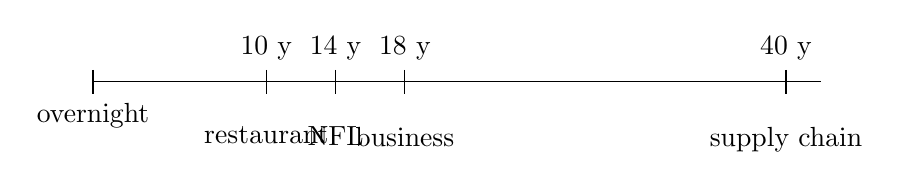
\begin{tikzpicture}[x=0.22cm,y=1cm]
\draw (0,0) -- (42,0);
\draw (0,0.15) -- (0,-0.15);
\node[below] at (0,-0.15) {overnight};
\foreach \x/\lab in {10/{10 y},14/{14 y},18/{18 y},40/{40 y}}{
  \draw (\x,0.15)--(\x,-0.15);
  \node[above] at (\x,0.15) {\lab};
}
\node[below] at (10,-0.45) {restaurant};
\node[below] at (14,-0.45) {NFL};
\node[below] at (18,-0.45) {business};
\node[below] at (40,-0.45) {supply chain};
\end{tikzpicture}
\caption{An editorial timeline of the horizons named in the lecture. The point is not numerical refinement but the repeated rejection of the ``overnight'' fantasy.}
\end{figure}

The speaker then explains why impatience is so destructive. People look at social media, do not know the truth of others' situations, and infer that the images they see dictate how they themselves ought to live. Hence the lecture's argument against speed is also an argument against imitation. In this formulation, financial failure is not only a matter of insufficient earnings; it is also a matter of adopting the wrong model of consumption.

\subsection{Question \& Answer}

\paragraph{Question.}
Why does wealth not arrive overnight?

\paragraph{Answer.}
Because the lecture's real sequence is
\begin{equation}
\text{learning} \longrightarrow \text{execution} \longrightarrow \text{scale},
\end{equation}
not
\begin{equation}
\text{visibility} \longrightarrow \text{wealth}.
\end{equation}
One studies under somebody who has already done the work, accepts that the learning phase does not pay like the mature phase, and only then converts borrowed knowledge into independent execution.

This is exactly the point the host extracts in his recap. He does not merely say ``be patient.'' He says: find experts, learn everything you can from them, and then apply and execute. The recap is important because it turns the interview from anecdote into method.

\section{Rock Bottom, Forward Motion, and Small-to-Large Scale}

The restaurant-owner interview deepens the lecture because it gives us a full arc from deprivation to operating scale. We are told not only that the speaker was broke, but that he slept in parking lots. The chapter should not smooth that away. The lecture uses it to explain why risk feels different at rock bottom.

\begin{align}
T^{\mathrm{restaurant}} &\approx 10\,\text{years},\\
Y_{\max}^{\mathrm{restaurant}} &\approx \$10\,\text{million},\\
N_{\mathrm{loc}} &= 5,\\
N_{\mathrm{emp}} &\in [85,100].
\end{align}

The turning-point logic is striking. When one is already at the bottom, the perceived downside of trying is reduced. The speaker says, in effect, what is left to lose? The lecture does not formalize this in the language of decision theory, but it clearly narrates a shift in the geometry of action. Once the worst has already been visited, motion becomes less terrifying.

\subsection{Question \& Answer}

\paragraph{Question.}
What is an actionable step when somebody is at rock bottom?

\paragraph{Answer.}
The answer given in the interview is specific and should remain specific: one must put God in the heart. The speaker presents this as the first practical reordering of life. From there the instruction is to go forward and to keep pushing. In the notes, we should preserve both parts of the answer. The first is spiritual in the speaker's own terms; the second is kinetic. One moves.

The same interview then turns from recovery to business scale. The story begins inside a gas station with what sounds like the owner plus one additional worker, and it ends with five locations and a staff between \(85\) and \(100\).

\paragraph{Worked scaling example.}
If we take ``me and one guy'' literally, the transcript suggests the rough path
\begin{align}
N_{\mathrm{loc}} &: 1 \to 5,\\
N_{\mathrm{emp}} &: 2 \to [85,100].
\end{align}
Hence the scale multipliers are
\begin{equation}
\frac{N_{\mathrm{loc,final}}}{N_{\mathrm{loc,initial}}} = 5,
\qquad
\frac{N_{\mathrm{emp,final}}}{N_{\mathrm{emp,initial}}} \in [42.5,50].
\end{equation}

This is not a full business model and should not be presented as one. It is simply a clean way to preserve what the lecture is doing verbally: showing that a very small starting operation can expand into something operationally substantial.

The interview then moves into education. The speaker's complaint about school is not merely anti-academic. It is a complaint about instruction that is not grounded in lived business formation. The proposed alternative is apprenticeship on the business side itself: wake up early, work in the operation, and keep working no matter how much money has already been made.

\section{Interruption, Mission, and the Arithmetic of Preservation}

The lecture is then interrupted by security. This moment is structurally important. It gives the host a chance to restate the mission of the channel and to place risk into the argument itself. ``Take the risk or lose the chance'' is not an extraneous slogan here. It is the bridge between the restaurant-owner's account of forward motion and the next large theme of the lecture.

The Von Miller interview begins with spectacular earnings, but the real lesson is not how to make a large amount of money. It is how not to lose it. The phrase that organizes the entire section is repeated almost comically: save bread.

\begin{align}
Y_{\max}^{\mathrm{NFL}} &= \$38\,\text{million},\\
T^{\mathrm{NFL}} &\approx 14\,\text{years}.
\end{align}

To give this part of the lecture some mathematical clarity, we introduce a minimal bookkeeping language.

\begin{definition}
Let \(Y_t\) be income during period \(t\), \(C_t\) consumption during that period, \(S_t\) retained savings, \(W_t\) wealth stock, and \(R_t\) the return generated by already retained capital.
\end{definition}

The host's recap and the interviewee's repeated instruction are naturally organized by the identities
\begin{align}
S_t &= Y_t - C_t,\\
W_{t+1} &= W_t + S_t + R_t.
\end{align}
Subtracting \(W_t\) from both sides gives the update rule
\begin{align}
\Delta W_t &= W_{t+1} - W_t \\
&= Y_t - C_t + R_t.
\end{align}

\paragraph{Worked derivation.}
\begin{enumerate}
\item Begin with income \(Y_t\).
\item Remove consumption to obtain retained savings \(S_t = Y_t - C_t\).
\item Add retained savings to the existing wealth stock \(W_t\).
\item Add the return \(R_t\) generated by capital already kept.
\item This yields \(W_{t+1} = W_t + S_t + R_t\), hence \(\Delta W_t = Y_t - C_t + R_t\).
\end{enumerate}

\begin{proposition}
High income by itself does not imply growth of wealth.
\end{proposition}

\begin{proof}
Under the update rule above, wealth growth requires
\[
\Delta W_t = Y_t - C_t + R_t.
\]
If consumption rises until it nearly absorbs income, so that \(C_t \approx Y_t\), then \(S_t \approx 0\) and therefore
\[
\Delta W_t \approx R_t.
\]
In that regime, extraordinary earnings do not automatically translate into durable accumulation. One must retain income as well as earn it.
\end{proof}

This is why the lecture immediately invokes cautionary stories of high earners who went broke. The arithmetic itself is simple. That simplicity is part of the point. The difficulty lies not in the formula, but in behavior.

\section{Long Careers and the Human Instrument}

The athlete interview does not stop at retention. It turns next to longevity, and here the lecture broadens its notion of preservation. One must preserve not only money, but also the human instrument that makes long-run earning possible.

The host asks what separates a professional player from the overwhelming majority who never reach that level. The answer is evolution and resilience. There were always others who were better, stronger, or faster. The durable asset was the ability to adapt.

The next question is then perfectly placed: how does one remain in the league for fourteen years when so many careers last only two or three? The response is again composite. There is grace, but there is also physical preparation, mental health, and self-awareness. The lecture treats these not as sentimental supplements, but as the tools of durability.

We may summarize the logic schematically as
\begin{equation}
\text{durability} \sim \text{resilience} + \text{preparation} + \text{self-awareness}.
\end{equation}
This is not a lecture-native equation. It is an editorial shorthand for the cluster of conditions the interview names.

What matters is the shift in scale. Earlier interviews showed us how people enter business, scale business, or recover from poverty. Here the question is how a human being sustains performance over a long horizon. The lecture keeps the same underlying form: the visible outcome only survives if the hidden mechanism is maintained.

\section{Early Risk and the Final Synthesis}

The final substantial interview returns to a smaller income scale, but it does not lower the argumentative stakes. We are again given a business horizon, another memory of not having enough food to eat, and then a closing concentration on early risk.

\begin{align}
T^{\mathrm{final}} &\approx 18\,\text{years},\\
Y_{\max}^{\mathrm{final}} &= \$500{,}000.
\end{align}

The older business owner says that nobody reaches full potential without taking risks early. He then describes his own crucial risk as stepping out on his own rather than remaining content with the paycheck of a large company. The final interview thus gathers together themes from earlier sections: honesty, risk, patience, hunger, and the refusal to stay passive.

\subsection{Question \& Answer}

\paragraph{Question.}
What early risk actually changes the shape of a life?

\paragraph{Answer.}
In this lecture, it is the risk of independent action. The interviewee does not describe a clever instrument or a hidden market inefficiency. He describes the decision to leave the security of serving another organization's success and to put one's own future at stake. The lecture presents this as the risk that reopens the space of possible outcomes.

The final answer to the question of becoming a millionaire in \(2024\) is therefore not a trick. It is a composite doctrine:
\begin{equation}
\text{wealth path} \approx \text{honesty} + \text{sacrifice} + \text{patience} + \text{risk} + \text{help-seeking}.
\end{equation}
This line is again editorial rather than spoken, but it does capture the closing cadence of the lecture. Work hard. Do not show off. Be honest. Reach out to people. Do not be afraid to ask for advice or support.

The point is not that every interviewee gives the same answer in the same words. The point is that by the end of the lecture, their answers have begun to converge.

\section{Summary}

The lecture begins with wealth as image and ends with wealth as mechanism. First we are taught that business stands on truth and the keeping of one's word. Then we are taught that scale requires time, apprenticeship, and freedom from imitative consumption. Next we are shown how poverty changes the relation to risk, and how even a very small operation can grow into a multi-location business. After that the lecture shifts to preservation: saving, retention, discipline, and the long-run update of wealth. Finally it closes by turning again to early risk, sacrifice, and the courage to ask for help.

If we compress the whole chapter into one sentence, it is this: large outcomes are real, but they are downstream of slower and less visible disciplines, and the lecture's real work is to make those disciplines visible.